Testing was performed mostly manually, and divided up into three parts. First, the API and models were tested independently, then, the Demo app's endpoints were tested, and finally, the API and the Demo App were tested together.

\subsection*{Stage 1 - API Testing}

The API was tested rigorously using Postman to perform testing. A new workspace was created, and the local testing deployment on port 5000 was tested. Primarily, the behaviour of the API when as it handles expected and unexpected input data was analyzed.

NOTE: All the testing was done in a development environment, and no testing was done on a production server due to finanical constraints of the team, and time contraints.
\\\\

\noindent
\begin{tabularx}{\textwidth}{|>{\raggedright\arraybackslash}p{4cm}|X|}
    \hline
    \textbf{Test Case ID:} & TC001 \\ \hline
    \textbf{Title:} & Validate \texttt{/predict route} \\ \hline
    \textbf{Precondition:} & The book dataset is loaded, the model is trained and dumped, the server is running and the recommendation model is deployed on port 5000. \\ \hline
    \textbf{Assumption:} & User submits a HTTP POST request to the \texttt{/predict} endpoint, from localhost. \\ \hline
\end{tabularx}

\noindent
\begin{tabularx}{\textwidth}{|>{\centering\arraybackslash}p{3cm}|>{\centering\arraybackslash}p{3cm}|X|}
    \hline
    \textbf{Number of Test Cases} & \textbf{Sub Test Case} & \textbf{Description and Expected Results} \\ \hline
    1 & TC001-1 & Input a valid book title and model name and expect the system to return the top 10 recommended books. \\ \hline
    2 & TC001-2 & Input only a valid book title, expects the API to return a descriptive error message. \\ \hline
    3 & TC001-3 & Inputs only a invalid book title and model, expects the API to return recommendations for the closest match \\ \hline
    4 & TC001-4 & Inputs a valid book title and invalid model name, expects the API to return a descriptive error message \\ \hline
    5 & TC001-4 & Inputs a valid book title and valid model name and some other junk data, expects the API to return a list of recommended books \\ \hline
\end{tabularx}

\noindent
\begin{tabularx}{\textwidth}{|>{\raggedright\arraybackslash}p{4cm}|X|}
    \hline
    \textbf{Expected Result:} & 
    \begin{itemize}
        \item TC001-1: The system should return a 201 output list of 10 recommended books related to the input title.
        \item TC001-2: The system should return a 404 JSON output with data \texttt{error: Book not found!}
        \item TC001-3: The system should return a 201 output list of 10 recommended books related to the input title.
        \item TC001-4: The system should return a 300 JSON output with data \texttt{error: Invalid model!}
        \item TC001-5: The system should return a 201 output list of 10 recommended books related to the input title, ignoring the other data.
    \end{itemize}
    \\ \hline
\end{tabularx}

\noindent
\begin{tabularx}{\textwidth}{|>{\raggedright\arraybackslash}p{4cm}|X|}
    \hline
    \textbf{Actual Result:} & 
    \begin{itemize}
        \item TC001-1: The system returned the correct list of 10 recommended books.
        \item TC001-2: The system displayed the appropriate error message
        \item TC001-3: The system displayed an appropriate error message.
        \item TC001-4: The system returned the appropriate error message
        \item TC001-5: The system returned the list of 10 recommendations.
    \end{itemize}
    \\ \hline
\end{tabularx}

\noindent
\begin{tabularx}{\textwidth}{|>{\raggedright\arraybackslash}p{4cm}|X|}
    \hline
    \textbf{Actual Output:} & 
    \begin{itemize}
        \item TC001-1: [List of 10 recommended books]
        \item TC001-2: [List of 10 recommended books with typo handling]
        \item TC001-3: "Error: Book title not found."
    \end{itemize}
    \\ \hline
    \textbf{Pass/Fail:} & 
    \begin{itemize}
        \item TC001-1: Pass
        \item TC001-2: Pass
        \item TC001-3: Pass
    \end{itemize}
    \\ \hline
\end{tabularx}

\begin{figure}[htbp]
    \centering
    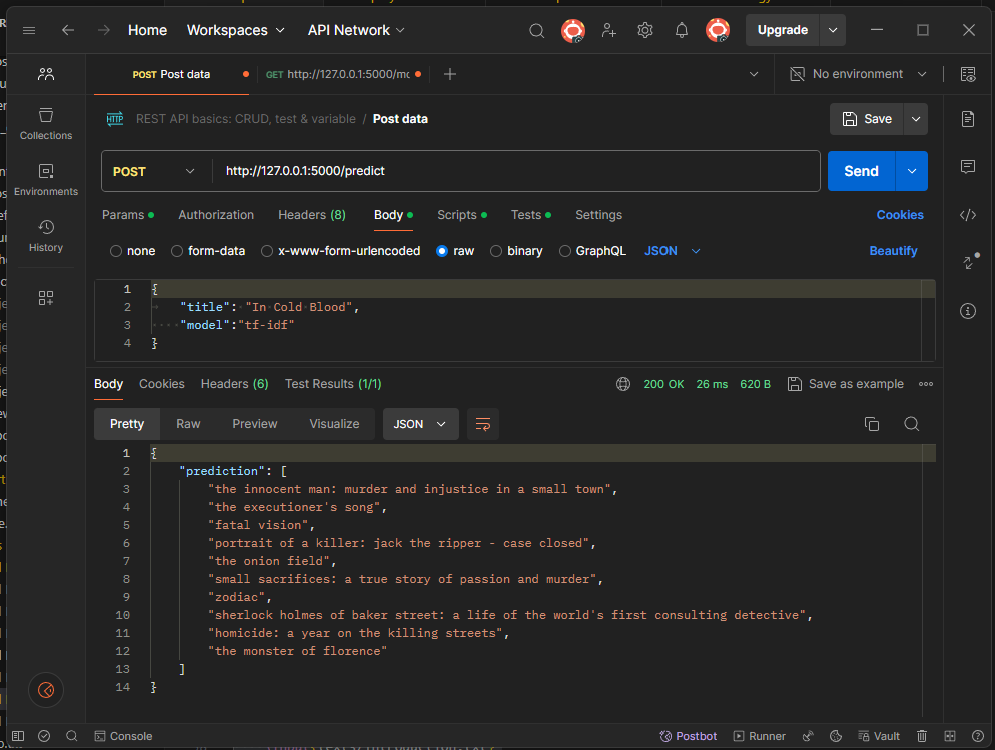
\includegraphics[width=1\textwidth]{../../assets/test_1.png}
    \caption{Test 1}
    \label{fig:test1}
\end{figure}
\begin{figure}[htbp]
    \centering
    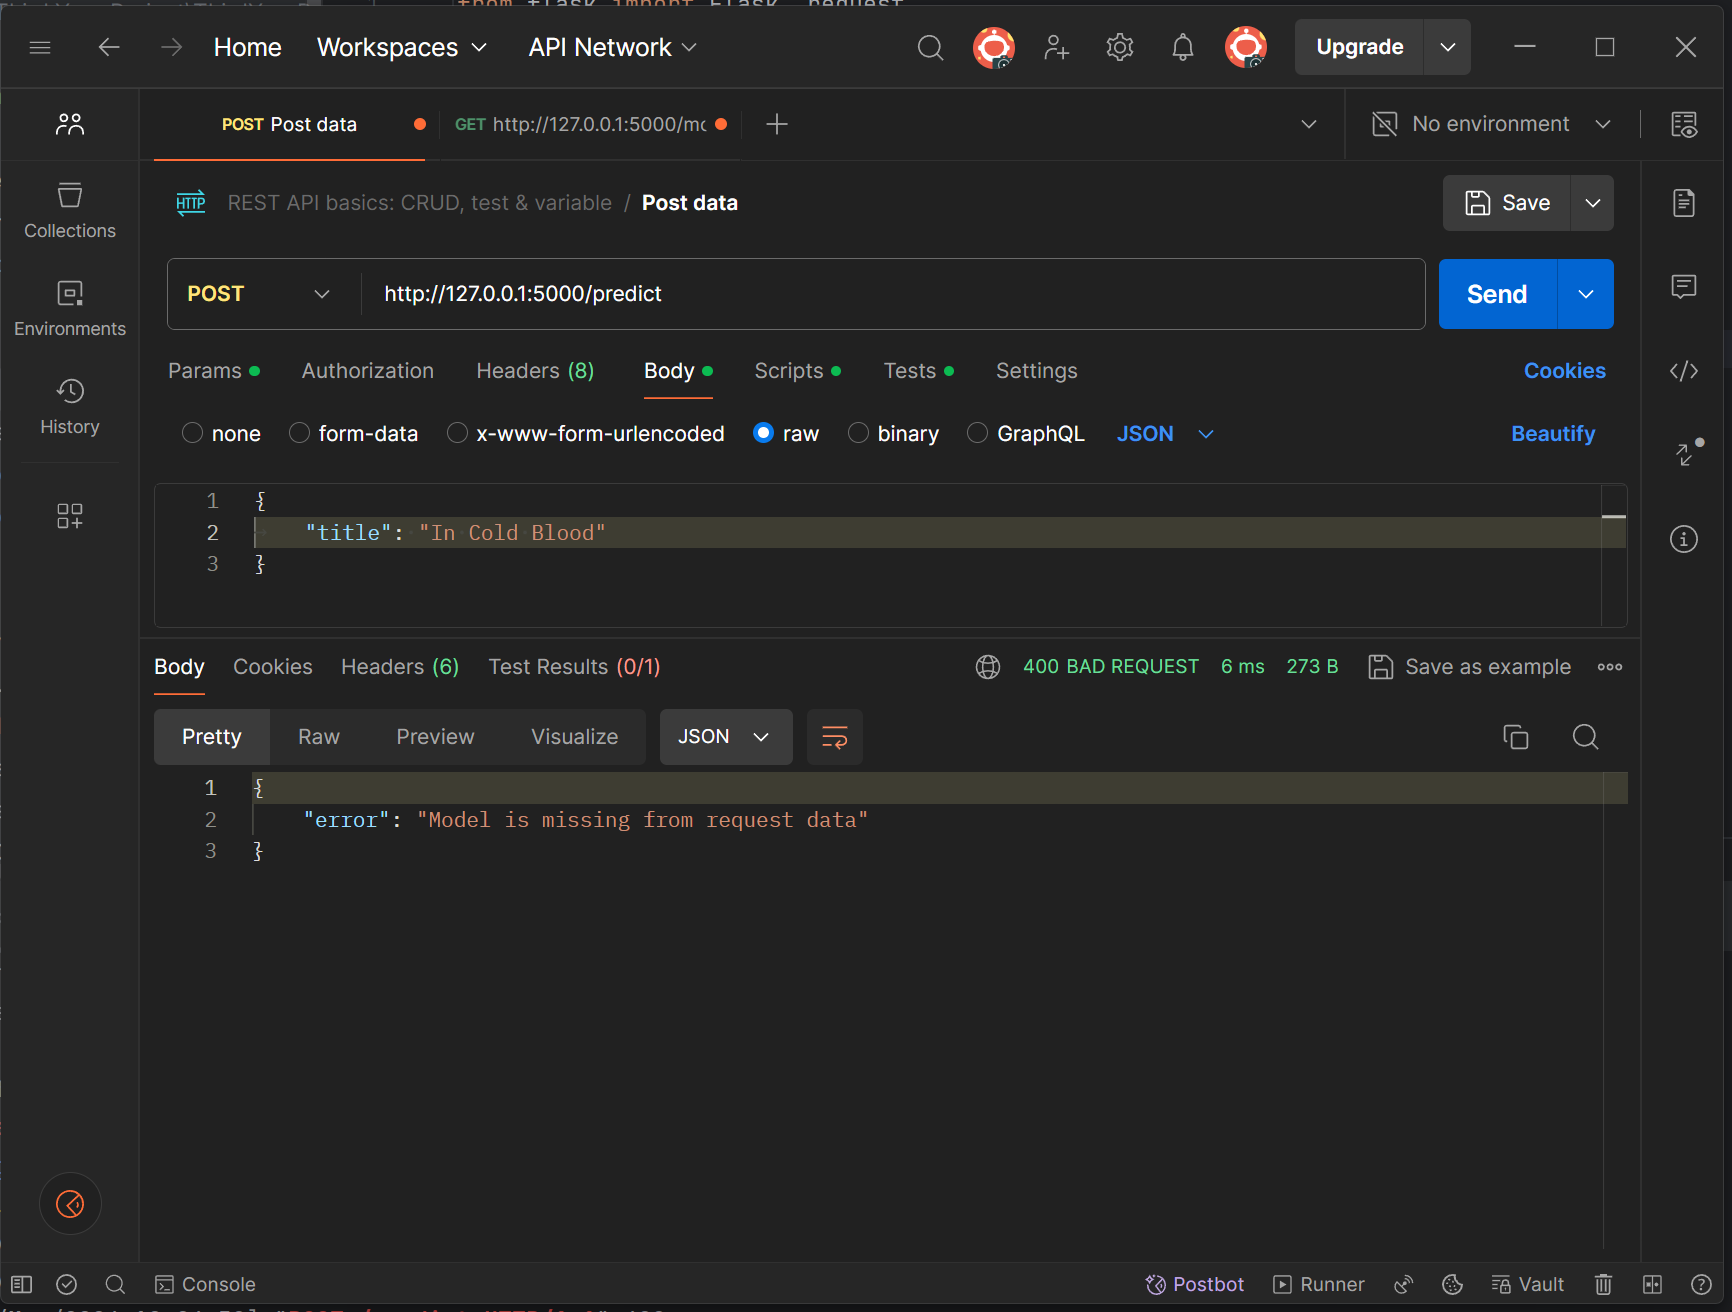
\includegraphics[width=1\textwidth]{../../assets/test_2.png}
    \caption{Test 2}
    \label{fig:test2}
\end{figure}
\begin{figure}[htbp]
    \centering
    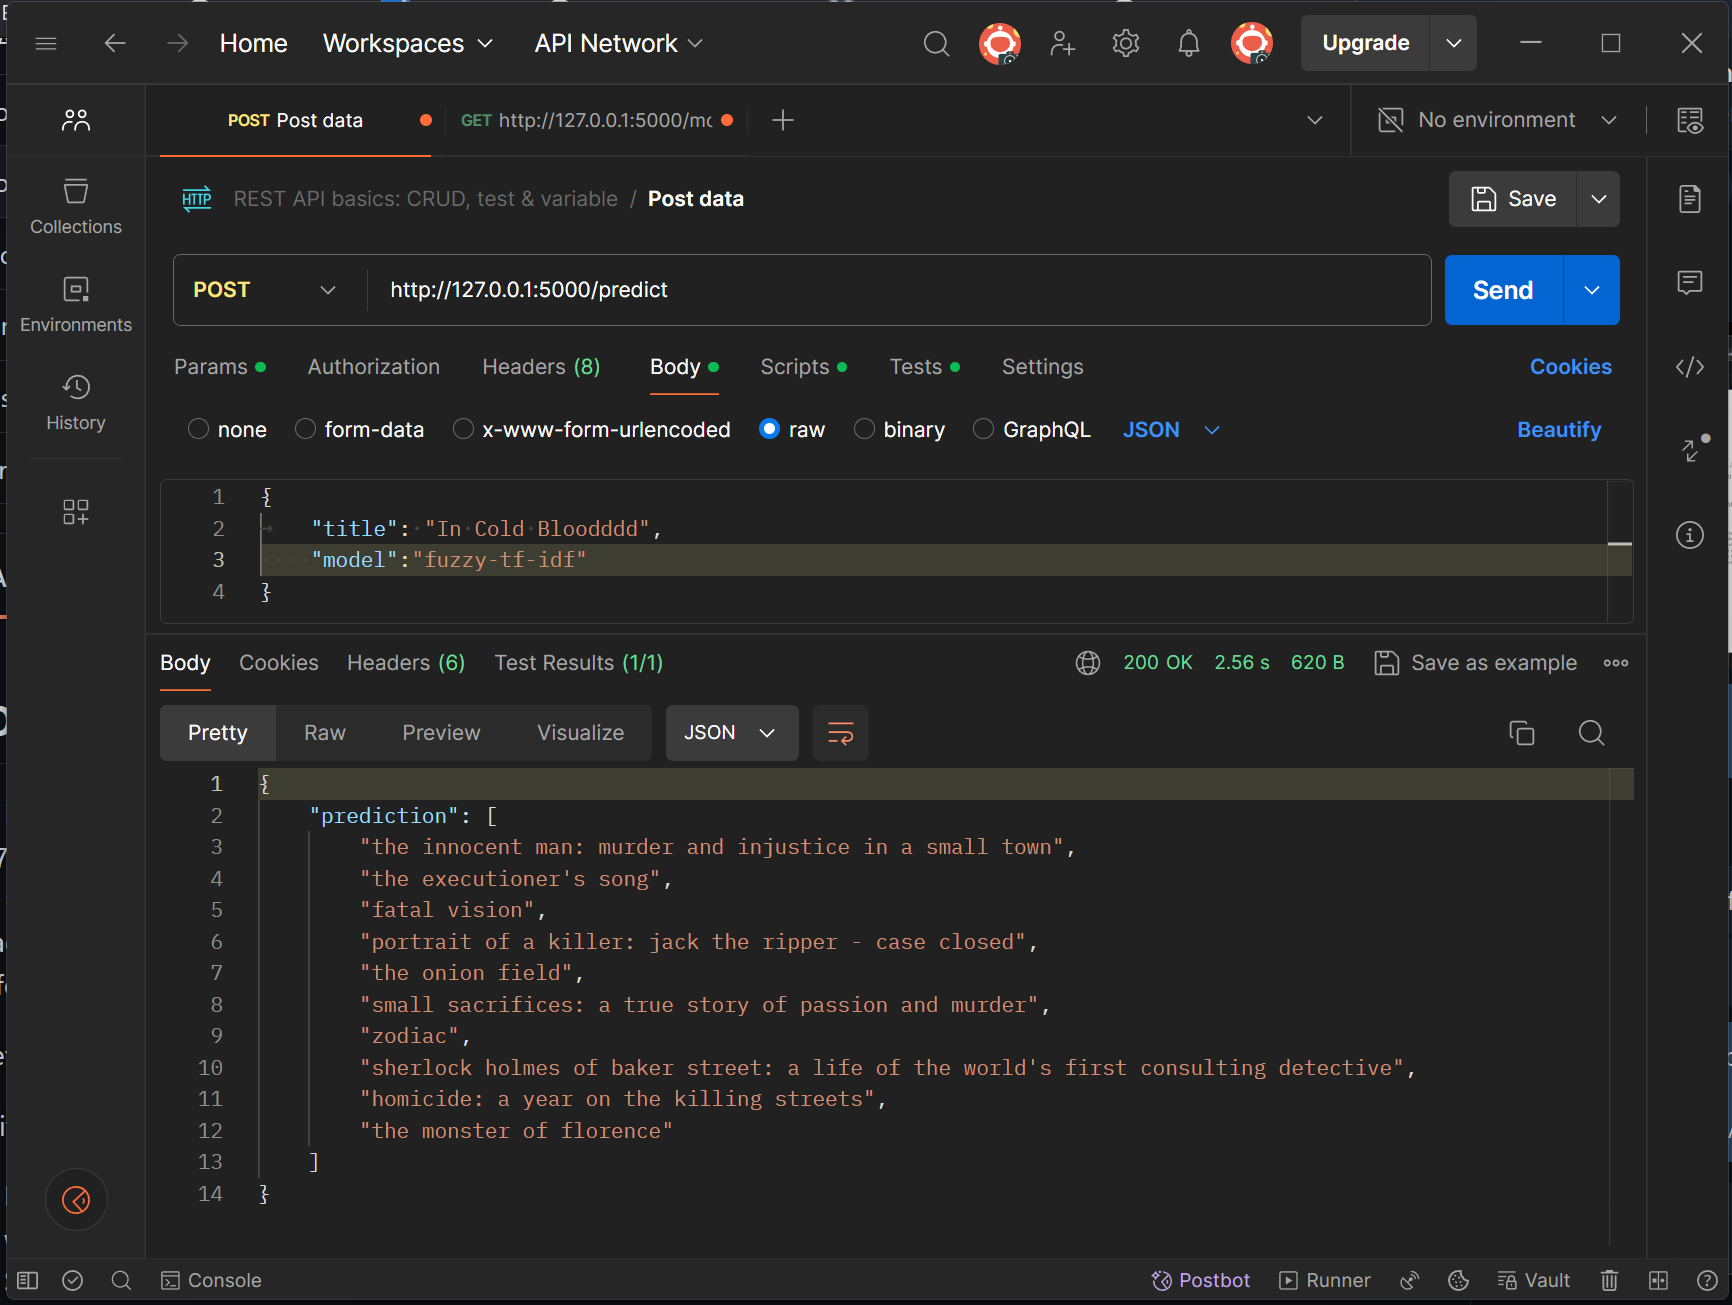
\includegraphics[width=1\textwidth]{../../assets/test_3.png}
    \caption{Test 3}
    \label{fig:test3}
\end{figure}
\begin{figure}[htbp]
    \centering
    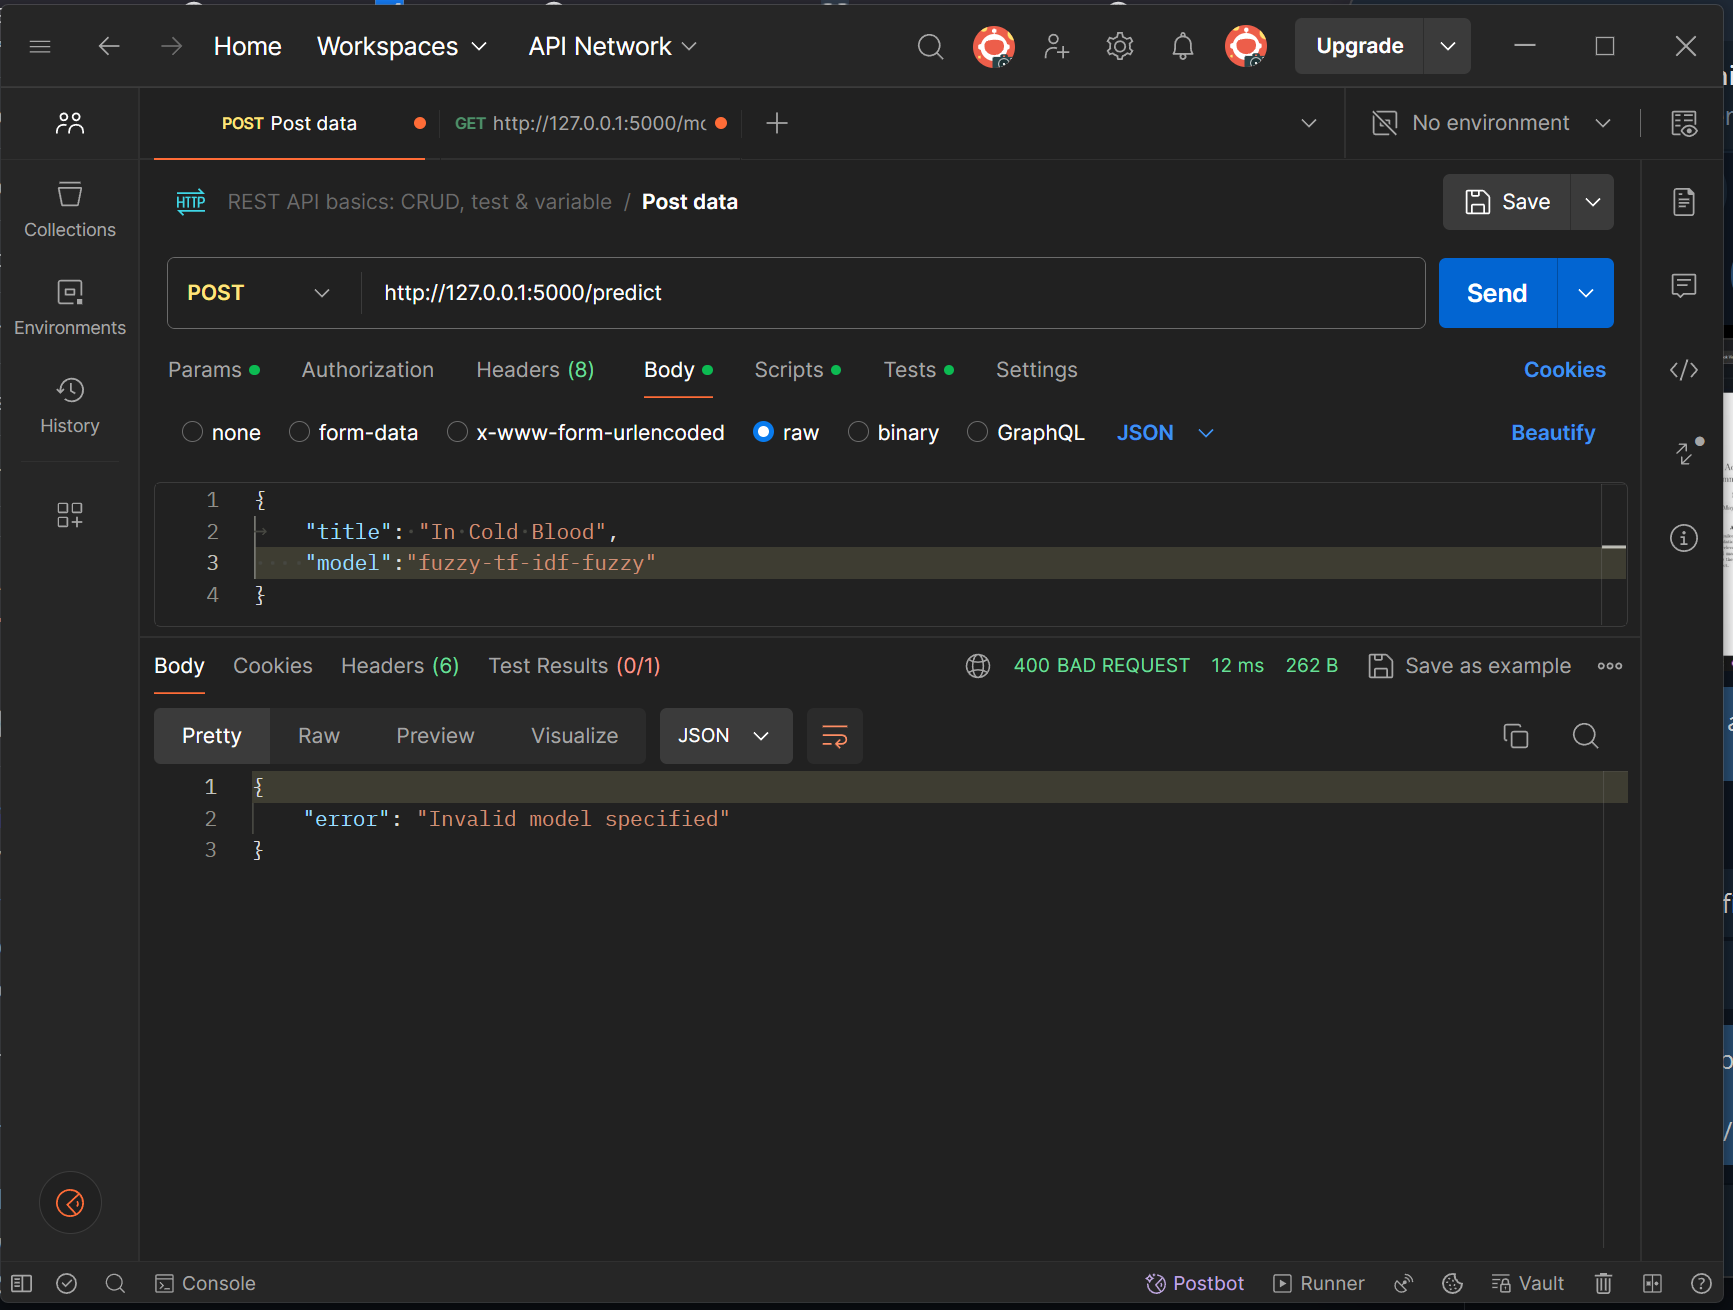
\includegraphics[width=1\textwidth]{../../assets/test_4.png}
    \caption{Test 4}
    \label{fig:test4}
\end{figure}
\begin{figure}[htbp]
    \centering
    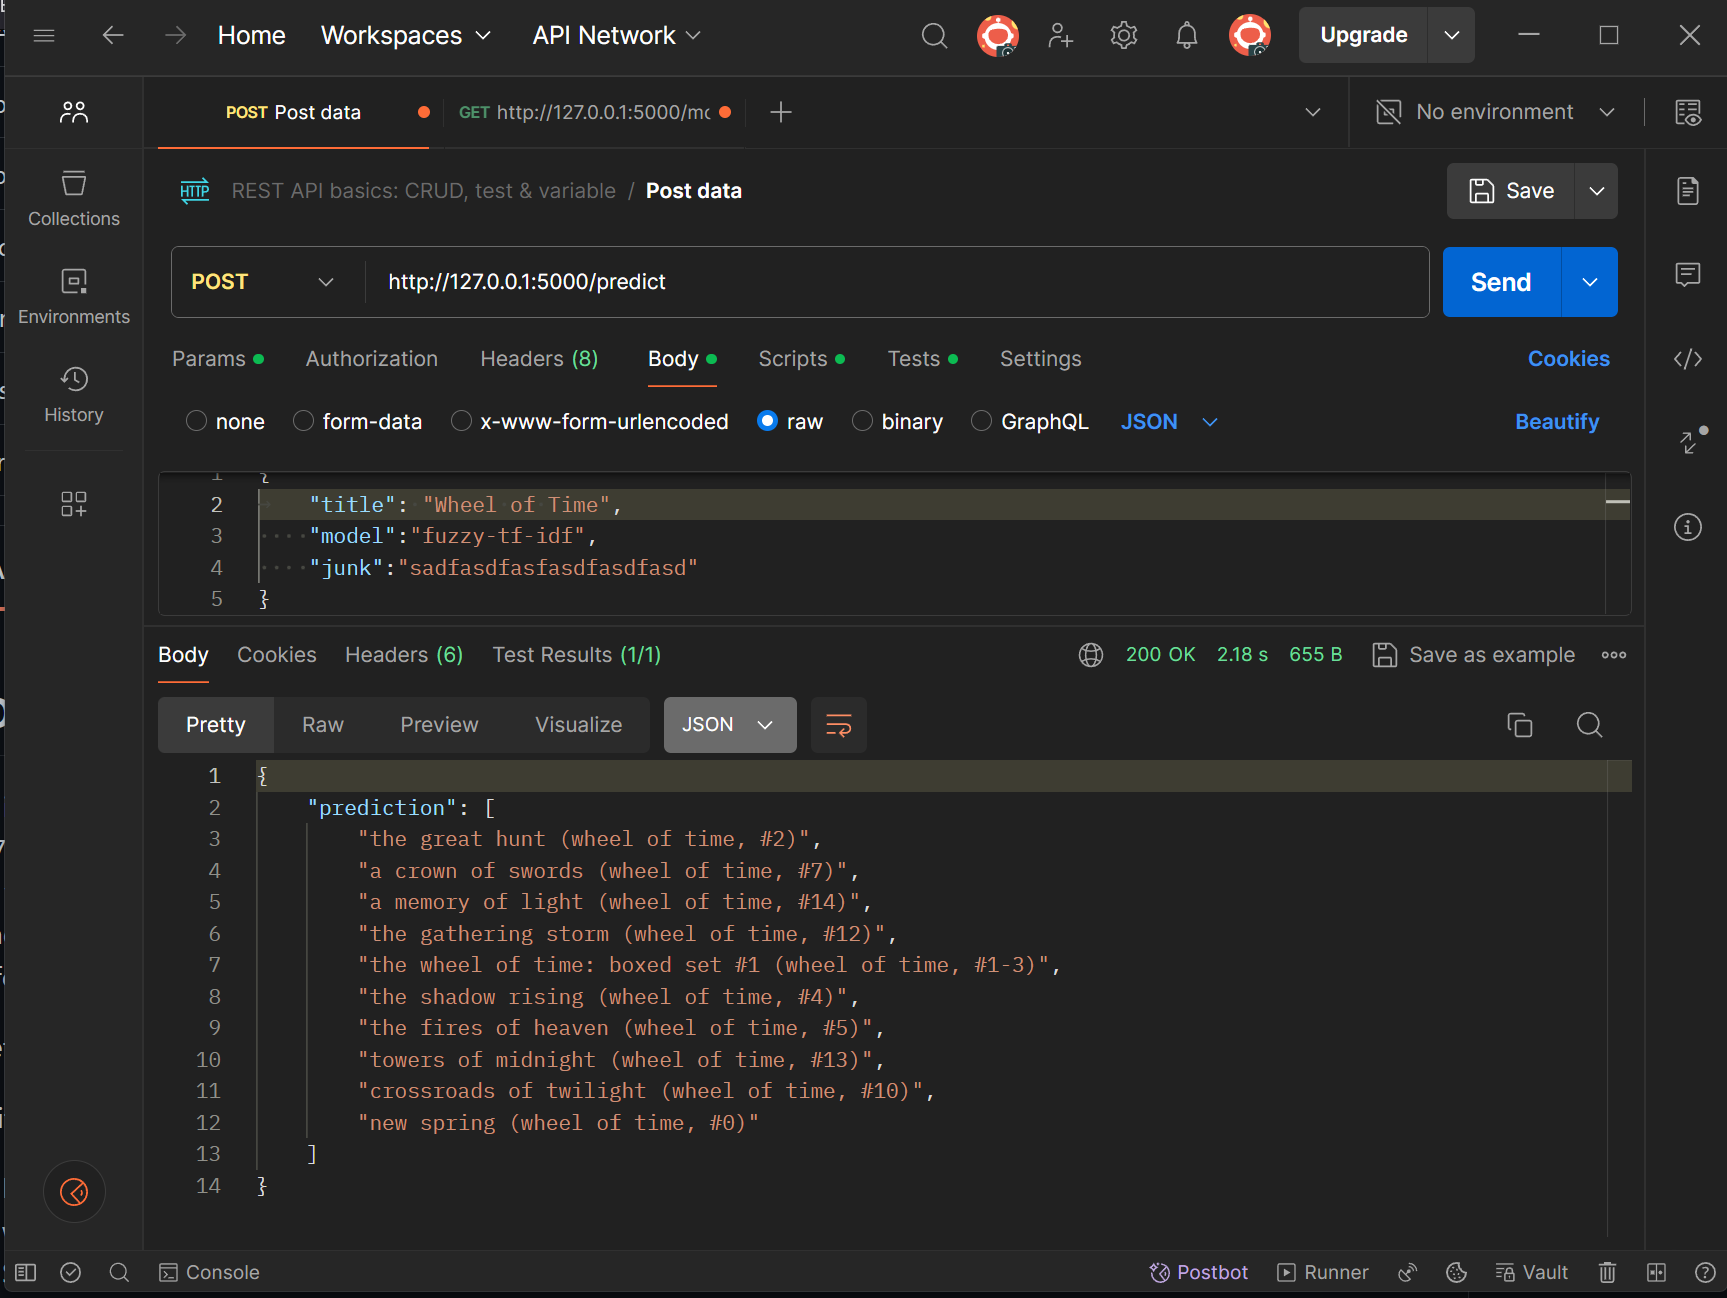
\includegraphics[width=1\textwidth]{../../assets/test_5.png}
    \caption{Test 5}
    \label{fig:test5}
\end{figure}


\noindent
\begin{tabularx}{\textwidth}{|>{\raggedright\arraybackslash}p{4cm}|X|}
    \hline
    \textbf{Test Case ID:} & TC002 \\ \hline
    \textbf{Title:} & User Interaction \\ \hline
    \textbf{Precondition:} & The recommendation model is deployed. \\ \hline
    \textbf{Assumption:} & User selects a book within the app. \\ \hline
\end{tabularx}

\noindent
\begin{tabularx}{\textwidth}{|>{\centering\arraybackslash}p{3cm}|>{\centering\arraybackslash}p{3cm}|X|}
    \hline
    \textbf{Number of Test Cases} & \textbf{Sub Test Case} & \textbf{Description and Expected Results} \\ \hline
    1 & TC002-1 & User selects a book and provides recommendation. \\ \hline
    2 & TC002-2 & App updates the interaction matrix. \\ \hline
\end{tabularx}

\noindent
\begin{tabularx}{\textwidth}{|>{\raggedright\arraybackslash}p{4cm}|X|}
    \hline
    \textbf{Expected Result:} & 
    \begin{itemize}
        \item The app should give correct results.
        \item Subsequent recommendations consider this new interaction.
    \end{itemize}
    \\ \hline
\end{tabularx}

\noindent
\begin{tabularx}{\textwidth}{|>{\raggedright\arraybackslash}p{4cm}|X|}
    \hline
    \textbf{Actual Result:} & 
    \begin{itemize}
        \item The app provided correct recommendations.
        \item Subsequent recommendations considered the new interaction.
    \end{itemize}
    \\ \hline
\end{tabularx}

\noindent
\begin{tabularx}{\textwidth}{|>{\raggedright\arraybackslash}p{4cm}|X|}
    \hline
    \textbf{Actual Output:} & 
    \begin{itemize}
        \item Correct recommendations were displayed.
        \item Interaction matrix was successfully updated.
    \end{itemize}
    \\ \hline
    \textbf{Pass/Fail:} & 
    \begin{itemize}
        \item TC002-1: Pass
        \item TC002-2: Pass
    \end{itemize}
    \\ \hline
\end{tabularx}

\noindent
\begin{tabularx}{\textwidth}{|>{\raggedright\arraybackslash}p{4cm}|X|}
    \hline
    \textbf{Test Case ID:} & TC001 \\ \hline
    \textbf{Title:} & Get Available Models \\ \hline
    \textbf{Precondition:} & The server is running and the models endpoint is accessible. \\ \hline
    \textbf{Assumption:} & None \\ \hline
\end{tabularx}

\noindent
\begin{tabularx}{\textwidth}{|>{\centering\arraybackslash}p{3cm}|>{\centering\arraybackslash}p{3cm}|X|}
    \hline
    \textbf{Number of Test Cases} & \textbf{Sub Test Case} & \textbf{Description and Expected Results} \\ \hline
    1 & TC001-1 & Send a GET request to the models endpoint with no data. Expected result: The server returns a list of available models. \\ \hline
    2 & TC001-2 & Send a request other than GET to the models endpoint. Expected result: The server returns an error. \\ \hline
\end{tabularx}

\noindent
\begin{tabularx}{\textwidth}{|>{\raggedright\arraybackslash}p{4cm}|X|}
    \hline
    \textbf{Expected Result:} & 
    \begin{itemize}
        \item For TC001-1: The server returns a list of available models.
        \item For TC001-2: The server returns an error.
    \end{itemize}
    \\ \hline
\end{tabularx}

\noindent
\begin{tabularx}{\textwidth}{|>{\raggedright\arraybackslash}p{4cm}|X|}
    \hline
    \textbf{Actual Result:} & 
    \begin{itemize}
        \item For TC001-1: The server returned a list of available models.
        \item For TC001-2: The server returned an error.
    \end{itemize}
    \\ \hline
\end{tabularx}

\noindent
\begin{tabularx}{\textwidth}{|>{\raggedright\arraybackslash}p{4cm}|X|}
    \hline
    \textbf{Actual Output:} & 
    \begin{itemize}
        \item For TC001-1: List of available models: ['model1', 'model2', ...].
        \item For TC001-2: Error message: "Method Not Allowed".
    \end{itemize}
    \\ \hline
    \textbf{Pass/Fail:} & 
    \begin{itemize}
        \item TC001-1: Pass
        \item TC001-2: Pass
    \end{itemize}
    \\ \hline
\end{tabularx}
\\\\

\begin{figure}[htbp]
    \centering
    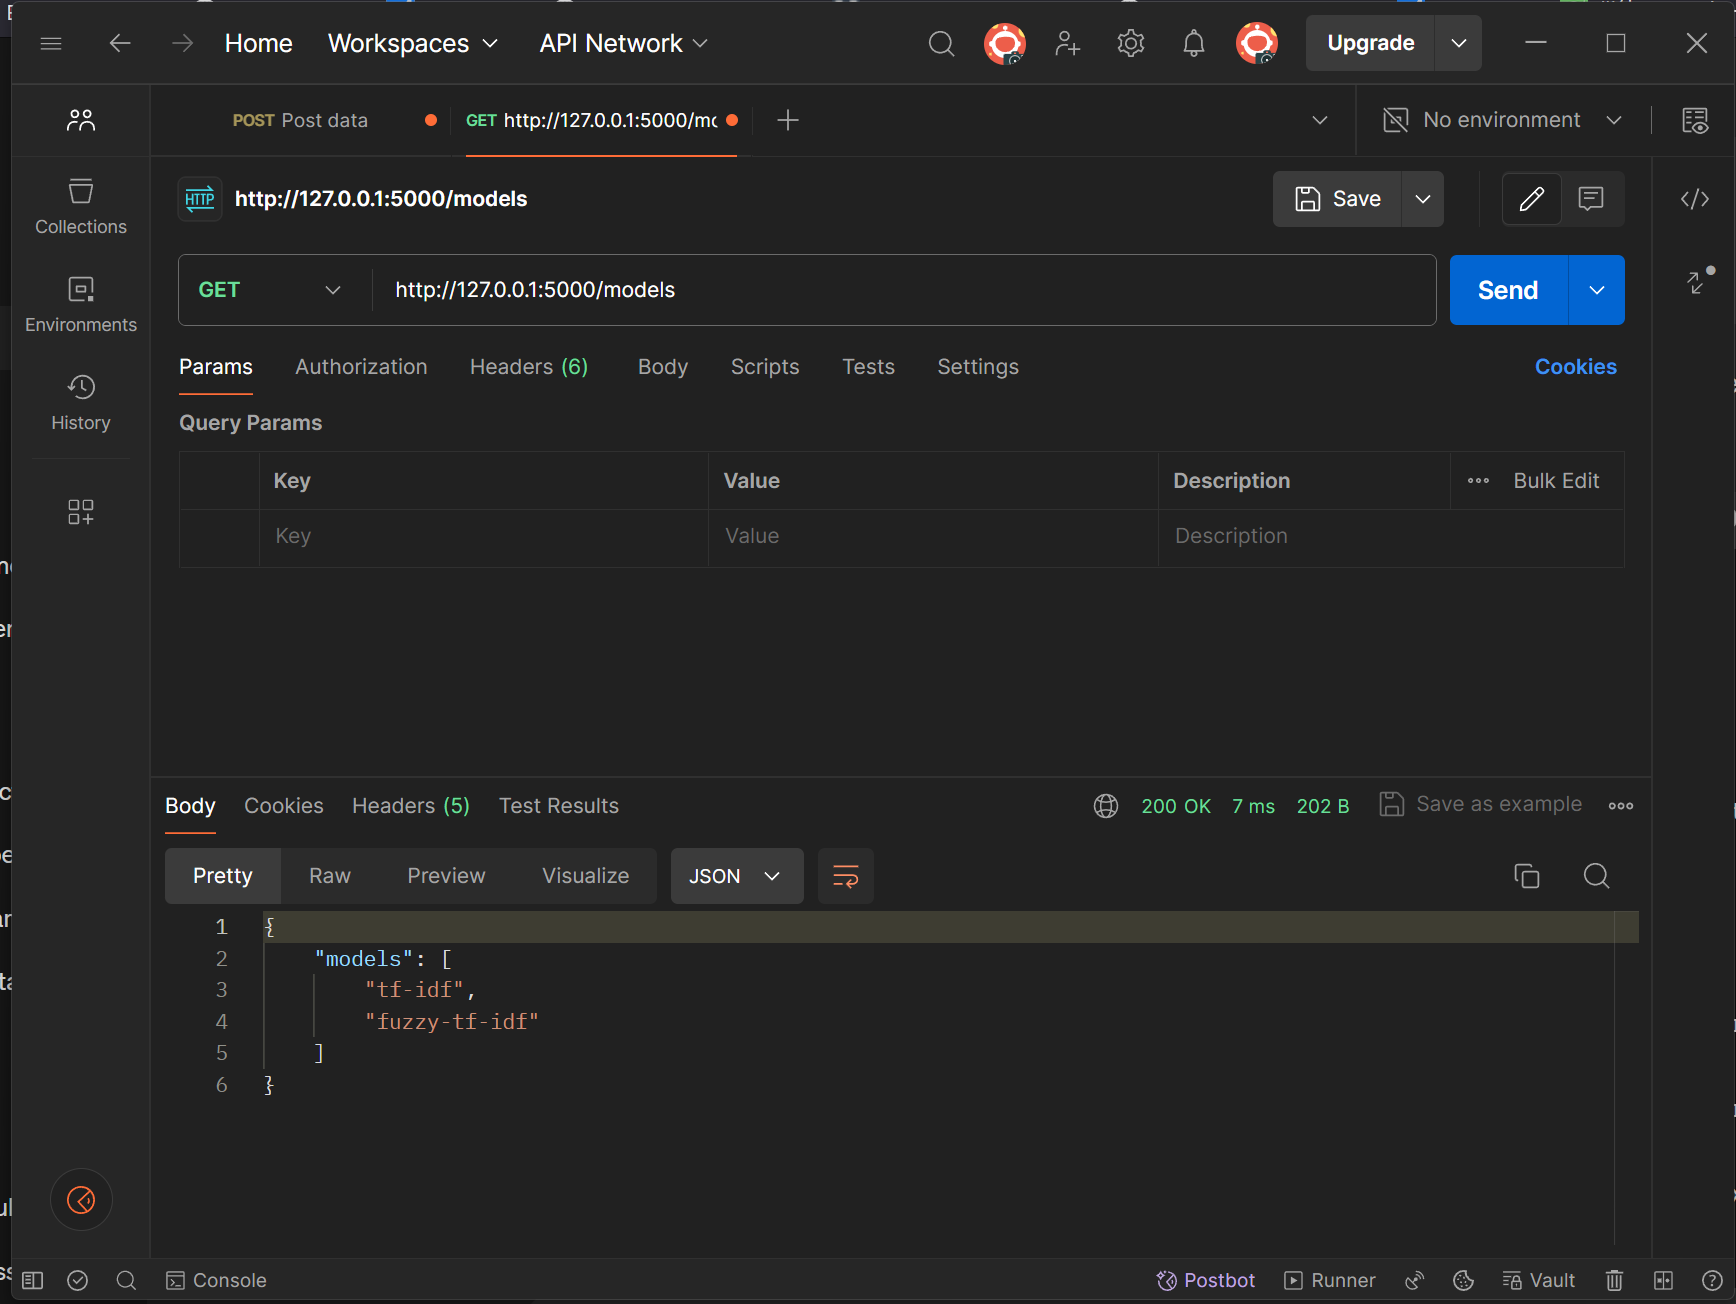
\includegraphics[width=1\textwidth]{../../assets/test_1_models.png}
    \caption{Test 1}
    \label{fig:test1models}
\end{figure}
\begin{figure}[htbp]
    \centering
    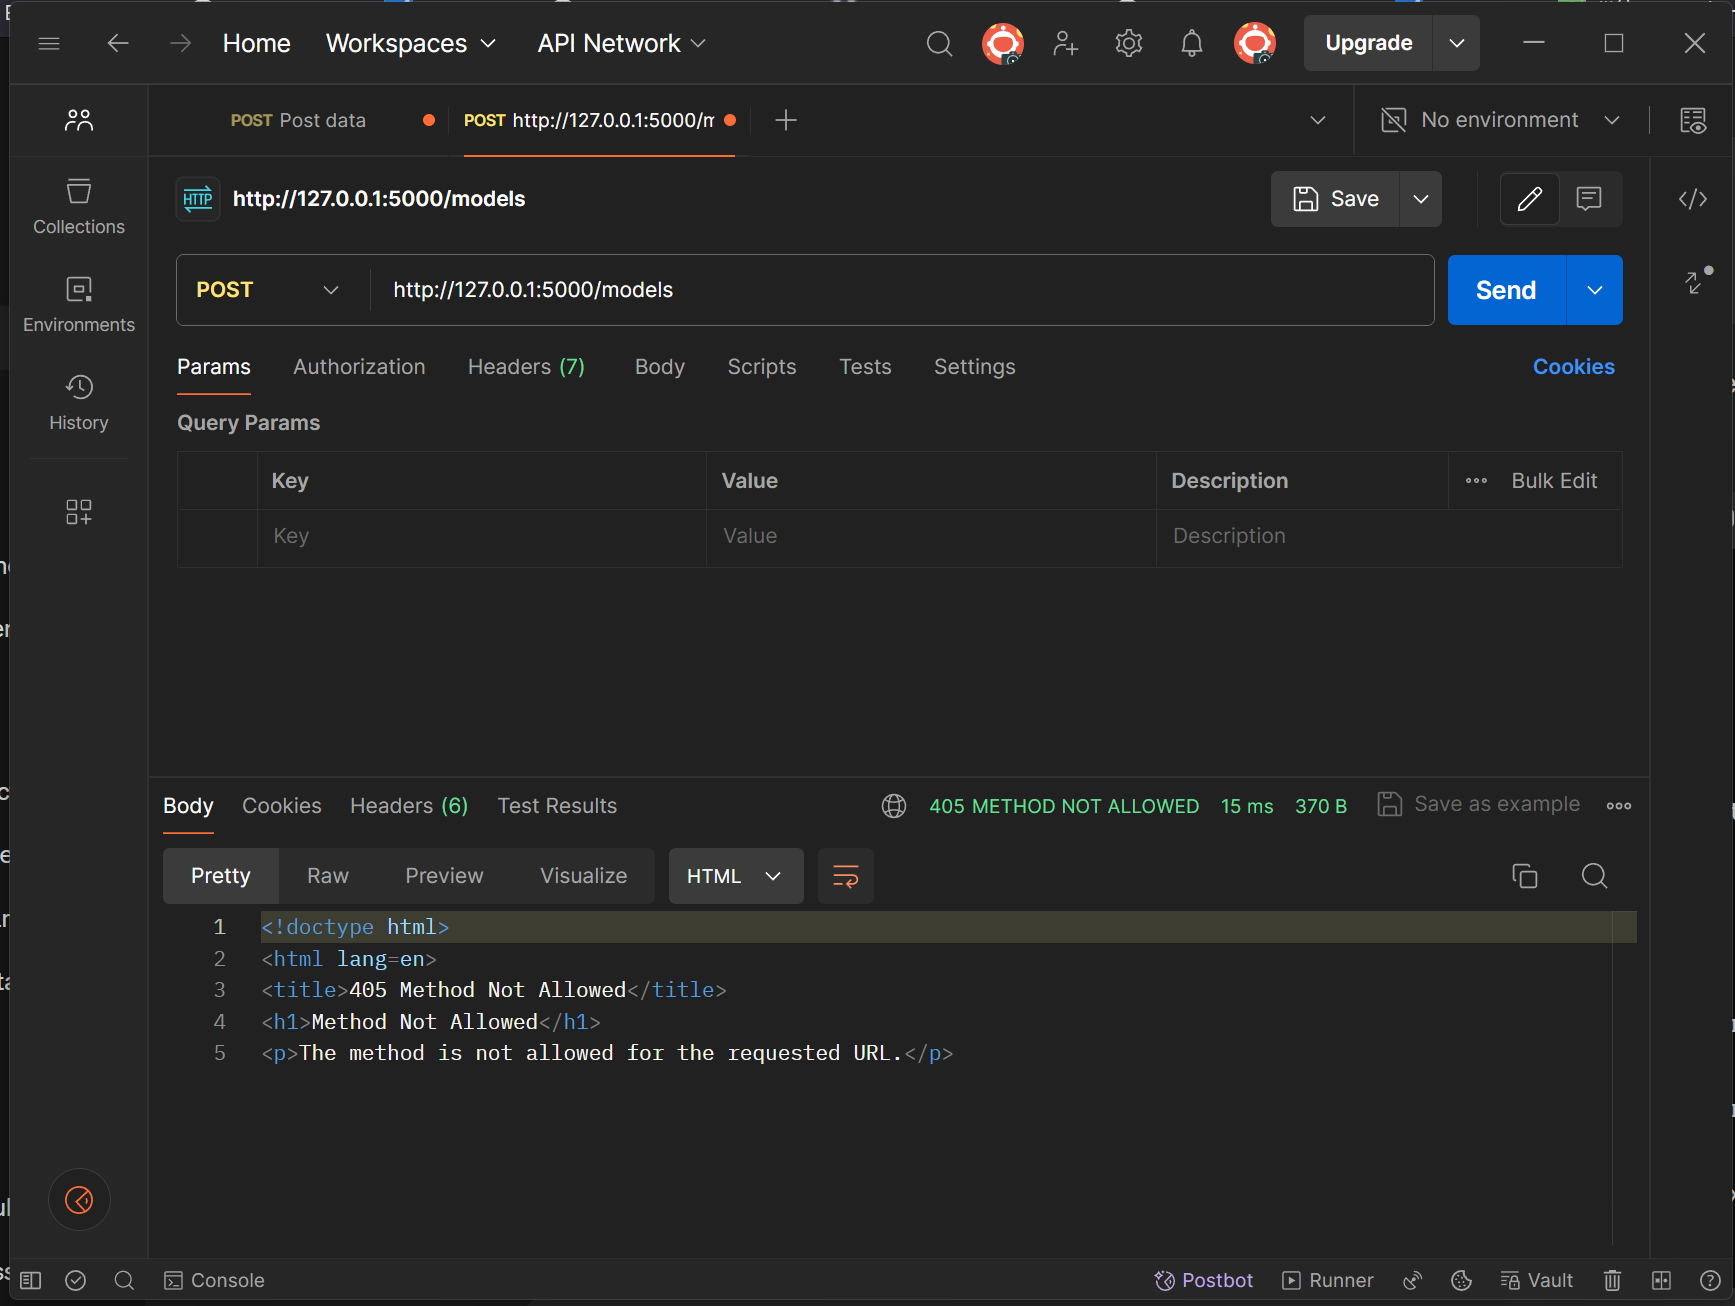
\includegraphics[width=1\textwidth]{../../assets/test_2_models.png}
    \caption{Test 2}
    \label{fig:test2models}
\end{figure}

\noindent
\begin{tabularx}{\textwidth}{|>{\raggedright\arraybackslash}p{4cm}|X|}
    \hline
    \textbf{Test Case ID:} & TC002 \\ \hline
    \textbf{Title:} & Book Recommendation via Next.js Application \\ \hline
    \textbf{Precondition:} & The Next.js application is running and accessible at port 3000 on the local machine. \\ \hline
    \textbf{Assumption:} & None \\ \hline
\end{tabularx}

\noindent
\begin{tabularx}{\textwidth}{|>{\centering\arraybackslash}p{3cm}|>{\centering\arraybackslash}p{3cm}|X|}
    \hline
    \textbf{Number of Test Cases} & \textbf{Sub Test Case} & \textbf{Description and Expected Results} \\ \hline
    1 & TC002-1 & Type in the name of a book and submit the form in the Next.js application. Expected result: The application returns a list of book recommendations. \\ \hline
\end{tabularx}

\noindent
\begin{tabularx}{\textwidth}{|>{\raggedright\arraybackslash}p{4cm}|X|}
    \hline
    \textbf{Expected Result:} & 
    \begin{itemize}
        \item For TC002-1: The Next.js application returns a list of book recommendations based on the input.
    \end{itemize}
    \\ \hline
\end{tabularx}

\noindent
\begin{tabularx}{\textwidth}{|>{\raggedright\arraybackslash}p{4cm}|X|}
    \hline
    \textbf{Actual Result:} & 
    \begin{itemize}
        \item For TC002-1: The Next.js application returned a list of book recommendations as expected.
    \end{itemize}
    \\ \hline
\end{tabularx}

\noindent
\begin{tabularx}{\textwidth}{|>{\raggedright\arraybackslash}p{4cm}|X|}
    \hline
    \textbf{Actual Output:} & 
    \begin{itemize}
        \item For TC002-1: List of recommended books: ['Book A', 'Book B', ...].
    \end{itemize}
    \\ \hline
    \textbf{Pass/Fail:} & 
    \begin{itemize}
        \item TC002-1: Pass
    \end{itemize}
    \\ \hline
\end{tabularx}

\begin{figure}[htbp]
    \centering
    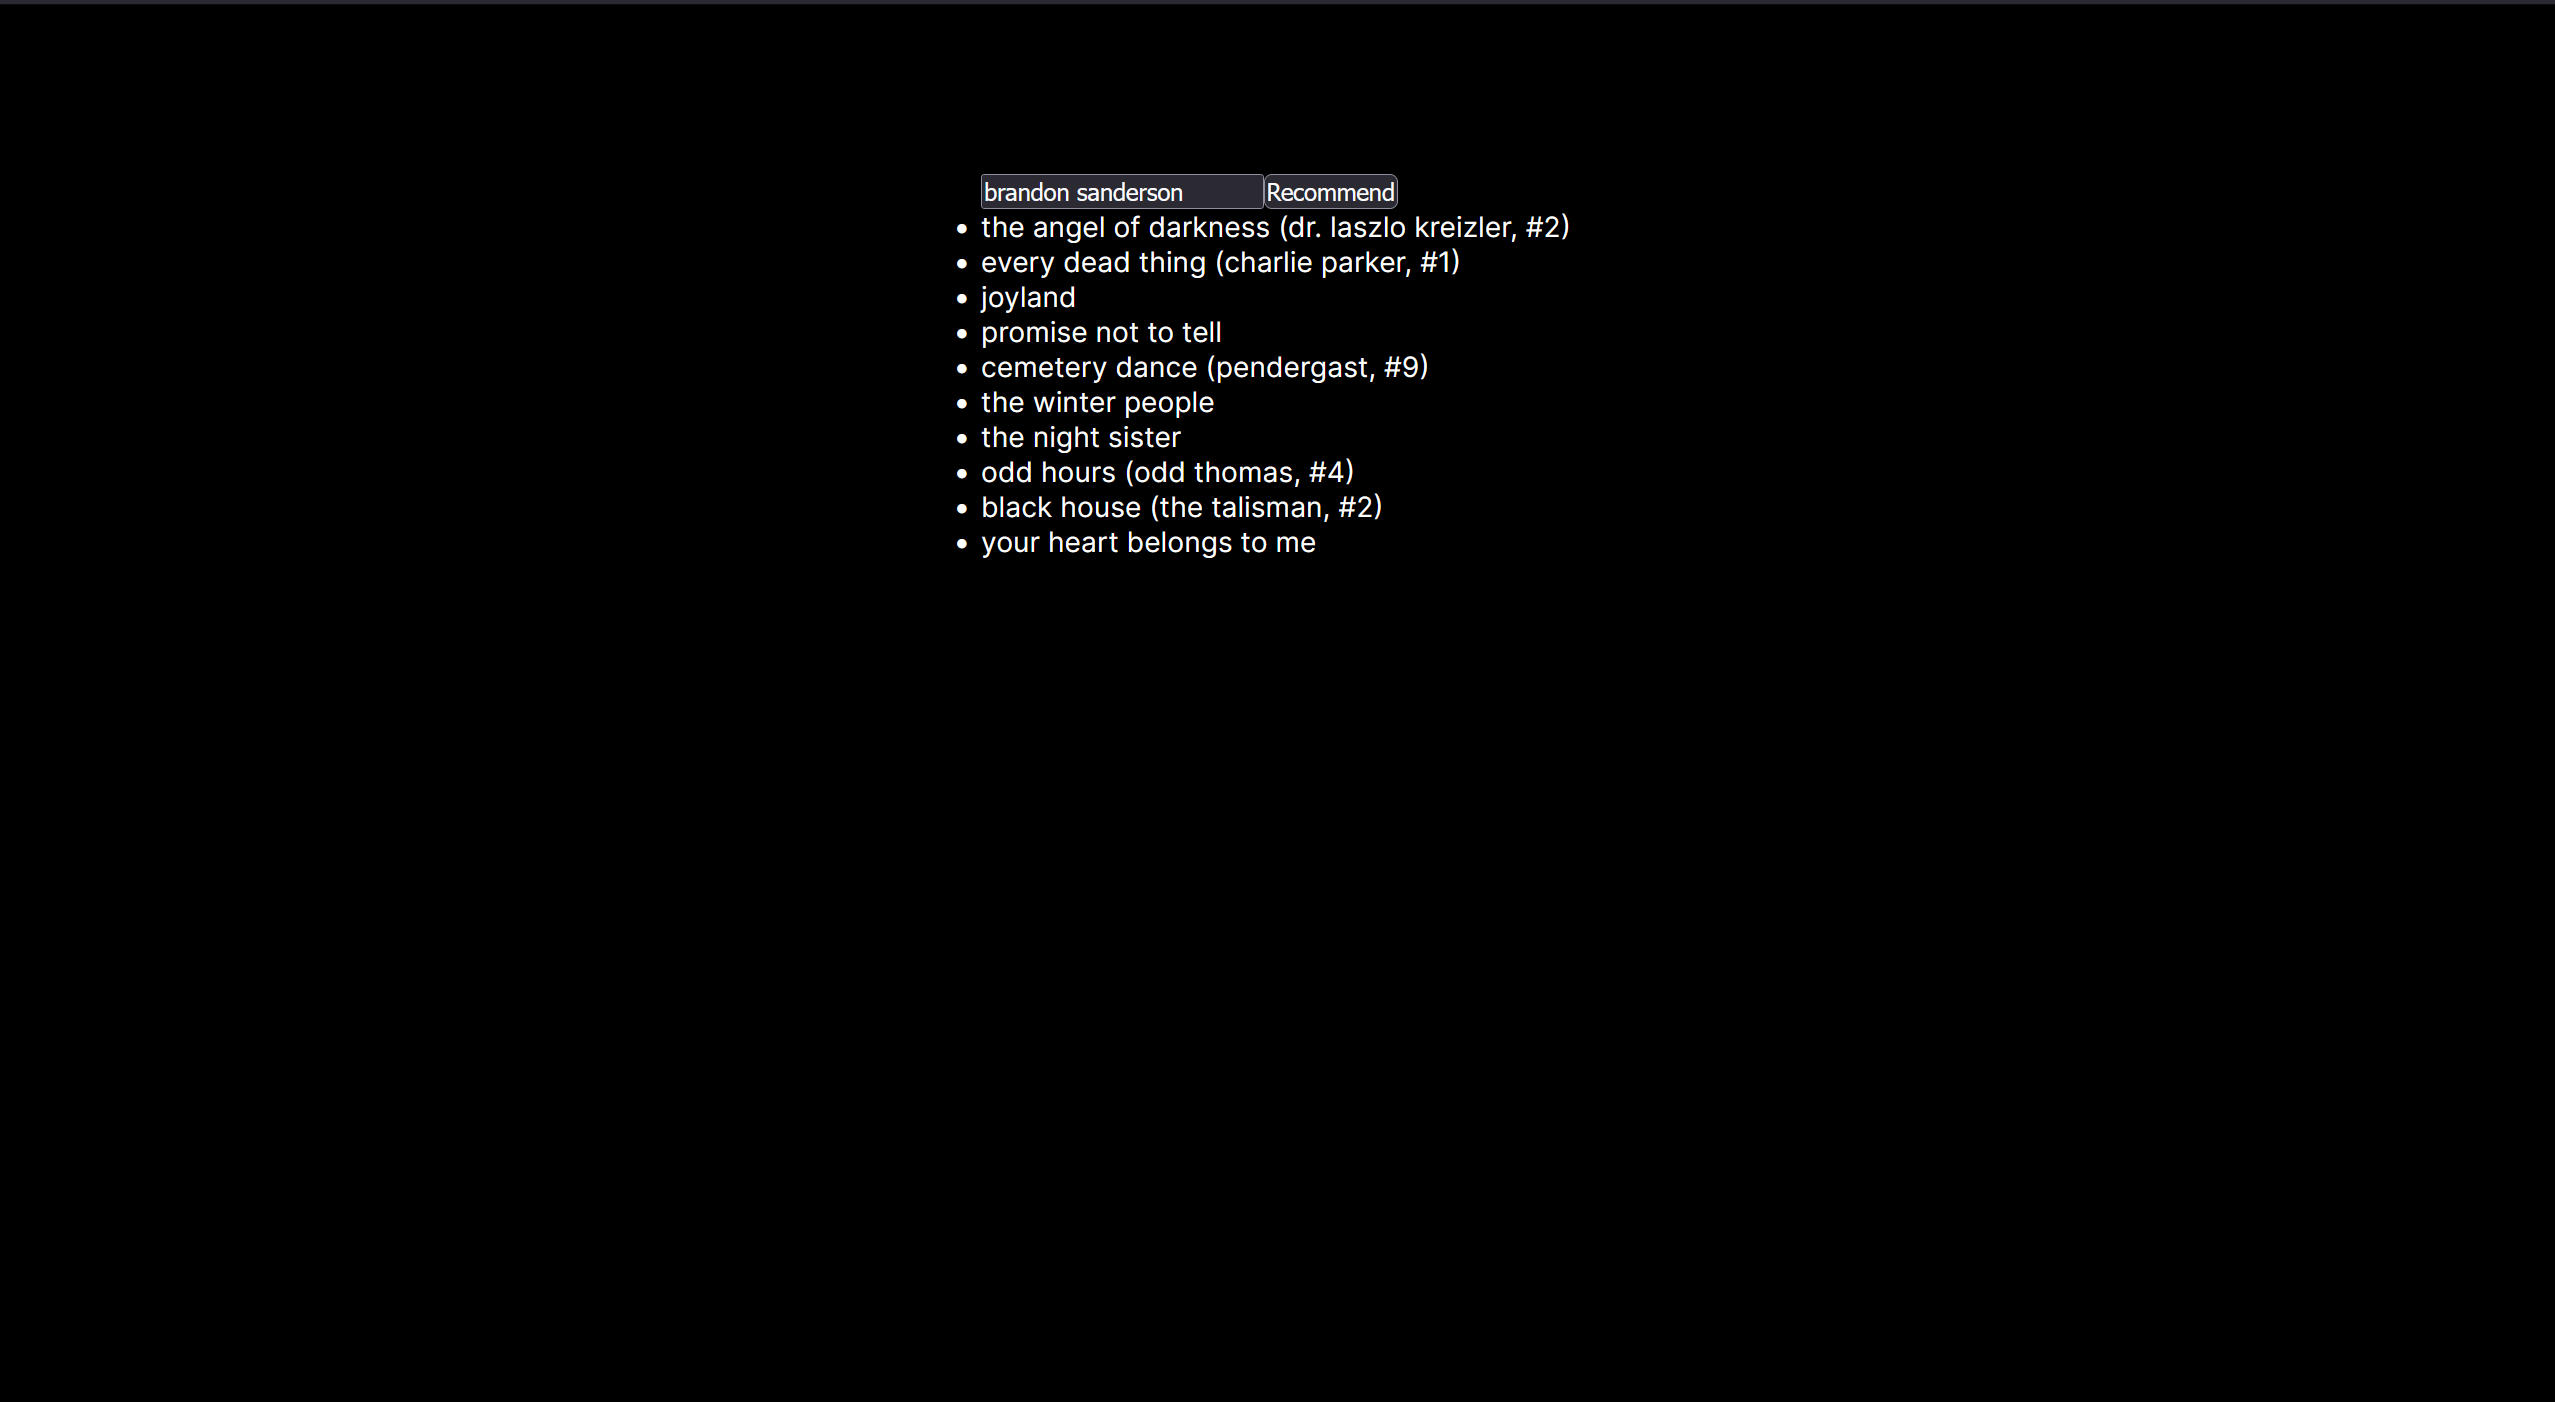
\includegraphics[width=1\textwidth]{../../assets/rudimentary_api_functionality.png}
    \caption{Rudimentary connection test}
    \label{fig:test2testApp}
\end{figure}